\section{Zusammenhänge von Auslastungs- und Potentialspielen}\label{sec:Auslastungsspiele}

\todo[inline]{Welche Endlichkeitsvoraussetzungen benötigt man hier jeweils?}

\todo{Mit Einleitung von Kapitel 1.3 vergleichen.}In \cite{RosenthalPotential} führte \citeauthor{RosenthalPotential} Auslastungsspiele als Klasse von endlichen Spielen ein, welche immer ein exaktes Potential (und damit ein Nash-Gleichgewicht) besitzen. Später zeigten \citeauthor{MonShap} in \cite[Theorem 3.2]{MonShap}, dass diese Klasse bis auf (kostenerhaltende) Isomorphie bereits \emph{alle} endlichen Spiele mit exaktem Potential umfasst. Zusammengefasst und etwas verallgemeinert gilt also:

\begin{satz}\label{satz:MondererShapley}
	Jedes $N$-Personen-Auslastungsspiel besitzt ein exaktes Potential und jedes exakte $N$-Personen-Potentialspiel ist äquivalent zu einem Auslastungsspiel.
\end{satz}

\begin{proof}
	Sei $\Gamma(M)$ ein beliebiges Auslastungsspiel. Dann definieren wir wie folgt die Rosenthal-Potentialfunktion:
		\[P: S \to \IR: s \mapsto \sum_{r \in R}\sum_{k=1}^{l_r(s)} g_r(k) \]
	Die Funktion ist wohldefiniert, da die insgesamt $N$ Spieler zusammen nur endlich viele Ressourcen nutzen können und daher beide Summen endlich sind. Sie ist ferner ein exaktes Potential, denn zu einem Strategieprofil $s \in S$ und einer weiteren Strategie $\hat{s}_i$ von Spieler $i$ gilt:
	\begin{align*}
		P(s) 	&- P(s\mid \hat{s}_i) = \sum_{r \in R}\sum_{k=1}^{l_r(s)} g_r(k) - \sum_{r \in R}\sum_{k=1}^{l_r(s\mid \hat{s}_i)} g_r(k) = \sum_{r \in s_i \setminus \hat{s}_i} g_r(l_r(s)) - \sum_{r \in \hat{s}_i \setminus s_i} g_r(l_r(s)+1) = \\
				&= \sum_{r \in s_i \setminus \hat{s}_i} g_r(l_r(s)) + \sum_{r \in s_i \cap \hat{s}_i} g_r(l_r(s)) - \sum_{r \in s_i \cap \hat{s}_i} g_r(l_r(s \mid \hat{s}_i)) - \sum_{r \in \hat{s}_i \setminus s_i} g_r(l_r(s\mid \hat{s}_i)) = \\
				&= \sum_{r \in s_i} g_r(l_r(s)) - \sum_{r \in \hat{s}_i} g_r(l_r(s\mid \hat{s}_i)) = c_i(s) - c_i(s \mid \hat{s}_i)
	\end{align*}
	
		
	Für die umgekehrte Richtung orientieren wir uns an dem Beweis in \cite[Theorem 1]{MultiPotGames}. Gegeben also ein Spiel $\Gamma = (I, X, (c_i)_{i\in i})$ mit einem exakten Potential $P$. Hierzu definieren wir folgendes Auslastungsmodell $M = (I, R, (S_i)_{i \in I}, (g_r)_{r \in R})$:
	\begin{itemize}
		\item $R \coloneqq R_K \cup R_D \subseteq \prod_{i \in I}\PSet(X_i)$, wobei $R_K \coloneqq \Set{\left(\{x_i\}\right)_{i \in I} | x_i \in X_i }$ und \\ $R_D \coloneqq \Set{(Y_i)_{i \in I} | \exists \hat{\imath} \in I: Y_{\hat{\imath}} = X_{\hat{\imath}}, \forall i \neq \hat{\imath}: \abs{X_i \setminus Y_i} = 1 }$.
		\item \[g_r(k) \coloneqq 
					\begin{cases}
						P(x), 					&r = \left(\{x_i\}\right)_{i \in I} \in R_k 													\text{ und } k=N \\
						c_{\hat{\imath}}(x) - P(x), 	&r = \left(X_i\setminus\{x_i\}\right)_{i \in I\setminus\hat{\imath}} \times X_{\hat{\imath}} \in R_D 	\text{ und } k=1 \\
						0,						&\text{sonst}
					\end{cases}\]
				\todo[inline]{Wohldefiniertheit!}
		\item $S_i \coloneqq \Set{ \Set{r \in R | x_i \in r_i} | x_i \in X_i }$
	\end{itemize}
	Die induzierten Lastfunktionen sind automatisch wohldefiniert, da die Spielermenge endlich ist, die Wohldefiniertheit der Kostenfunktionen $d_i$ folgt dann aus dem Beweis der Äquivalenz der Spiele $\Gamma$ und $\Gamma(M)$. Dazu betrachten wir den Morphismus $(\id, \phi): \Gamma \to \Gamma(M)$, wobei $\phi_i(x) \coloneqq s(x_i) \coloneqq \{r \in R \mid x_i \in r_i\}$. Dieser ist offenbar bijektiv auf allen Mengen und zudem kostenerhaltend, denn es gilt:
	\begin{align*}
		d_{\hat{\imath}}(\phi(x)) 	&=\sum_{r \in \phi(x)_{\hat{\imath}} = \phi_{\hat{\imath}}(x_{\hat{\imath}})} g_r(l_r(\phi(x))) = \\
		&=\sum_{r \in R_K: x_{\hat{\imath}} \in r_{\hat{\imath}}} g_r(\underbrace{l_r(\phi(x))}_{= N \iff r = \left(\{x_i\}\right)_{i \in I}}) + \sum_{r \in R_D: x_{\hat{\imath}} \in r_i} g_r(\underbrace{l_r(\phi(x))}_{=1 \iff r = \left(X_i\setminus\{x_i\}\right)_{i \in I\setminus\hat{\imath}} \times X_{\hat{\imath}}}) = \\
		&=g_{\left(\{x_i\}\right)_{i \in I}}(N) + g_{\left(X_i\setminus\{x_i\}\right)_{i \in I\setminus\hat{\imath}} \times X_{\hat{\imath}}}(1) = \\
		&=P(x) + c_{\hat{\imath}}(x) - P(x) = c_{\hat{\imath}}(x) \qedhere									
		\end{align*}
\end{proof}

\begin{bem}
	Berücksichtigt man nur die Ressourcen aus $R_K$, so erhält man ein Koordinationsspiel, nimmt man nur die aus $R_D$ so erhält man ein Dummy-Spiel. Aus dieser Beobachtung ergibt sich der in \cite{KoordDummy} beschriebene alternative Beweis für die Rückrichtung: Man zerlegt das exakte Potentialspiel zunächst in ein Koordinations- und ein Dummyspiel (siehe \Cref{satz:CharExPotAlt}), konstruiert für jedes der beiden ein äquivalentes Auslastungsspiel (mit Ressourcenmengen $R_K$ bzw. $R_D$) und erhält schließlich die Summe der beiden Auslastungsspiele als zum Ausgangsspiel kostenerhaltend isomorphes Auslastungsspiel.
\end{bem}

Auslastungsspiele sind also nicht nur \emph{ein} Beispiel für Spiele mit exaktem Potential, sondern in gewissem Sinne (nämlich bis auf Isomorphie) sogar \emph{das} Beispiel für solche Spiele. Eine naheliegende Frage ist nun, ob es ähnliche Klassen von \glqq auslastungsartigen\grqq{} Spielen gibt, welche genau den Spielen mit allgemeineren Potentialen entsprechen. Im Folgenden werden wir versuchen eine zu gewichteten Potentialspielen passende Verallgemeinerung von Auslastungsspielen zu finden.

\subsection{Von ungewichtet zu gewichtet}

\subsubsection{Gewichtete Auslastungsspiele}

Für gewichtete Auslastungsspiele zeigen \citeauthor{CharExGewPotinWCG} in \cite[Theorem 3.9]{CharExGewPotinWCG}, dass die einzigen beiden Klassen stetiger Funktionen, die (als Kostenfunktionen verwendet) ausschließlich endliche Spiele mit gewichtetem Potential erzeugen, affin lineare Funktionen bzw. exponentielle Funktionen (mit gemeinsamem Exponenten) sind:

\begin{satz}\label{satz:CharExGewPotinWCG}
	Gegeben eine Menge von stetigen Funktionen $C$. Dann besitzt genau dann jedes endliche gewichtete Auslastungsspiel, welches nur Funktionen aus $C$ als Kostenfunktionen verwendet, ein gewichtetes Potential, wenn $C$
	\begin{itemize}
		\item entweder ausschließlich affin lineare Funktionen enthält\todo{Fälle: Exaktes Potential/gewichtetes Potential unterscheiden}
		\item oder ausschließlich Funktionen der Form $c(l) = a_c\cdot b^l + d_c$ enthält.
	\end{itemize}
\end{satz}

In \cite[Theorem 5.1]{CharExNGinWCG} zeigen \citeauthor{CharExNGinWCG} weiter, dass diese beiden Klassen von Kostenfunktionen unter allen Klassen \emph{stetiger} Funktionen gleichzeitig auch die einzigen sind, die die Existenz eines Nash-Gleichgewichtes garantieren.\footnote{zudem sind es auch noch die einzigen Klassen, welche für jedes gewichtete Auslastungsspiel das Erfüllen der FIP sicherstellen.}

Da nun für endliche Spiele alle der in \Cref{sec:Potentiale} definierten Potentiale die Existenz eines Nash-Gleichgewichtes garantieren, folgt hiermit direkt, dass es auch für die allgemeineren Potentialbegriffe keine größeren oder anderen Klassen von stetigen Funktionen gibt, die immer die Existenz eines entsprechenden Potentials sicher stellen.

Zusammen zeigen diese beiden Sätze bereits deutlich, dass der Schritt vom ungewichteten Fall zum gewichteten auf Seite der Auslastungsspiele erheblich größer ist als auf Seite der Potentiale. Tatsächlich zeigt \citeauthor{ReprOfFiniteGamesAsNCG} in \cite{ReprOfFiniteGamesAsNCG}, dass dieser Verallgemeinerungsschritt für Auslastungsspiele bereits der größtmögliche ist, denn es gilt:

\begin{satz}\label{satz:JedesSpielGewAusl}
	Jedes endliche Spiel ist äquivalent zu einem gewichteten Auslastungsspiel \todo{(sogar Netzwerkauslastungsspiel mit ...)}.
\end{satz}

Die Menge der gewichteten Auslastungsspiele umfasst also (bis auf kostenerhaltende Isomorphie) bereits \emph{alle} (endlichen) Spiele in strategischer Form. Möchte man daher eine wirklich analoge Verallgemeinerung von Auslastungsspielen passend zu gewichteten Potentialspielen finden, muss man also andere Varianten betrachten Gewichte ins Spiel zu bringen. In \Cref{def:gewAuslastungsspiel} hatten wir bereits zwei solche gesehen, welche wir nun näher untersuchen wollen:

\subsubsection{Lastgewichtete Auslastungsspiele}

Die erste alternative Klasse von Auslastungsspielen sind die lastgewichteten Auslastungsspiele. \citeauthor{CharExGewPotinWCG} beobachten in \cite{CharExGewPotinWCG}, dass lastgewichtete Auslastungsspiele (die dort als normalisierte Auslastungsspiele bezeichnet werden) zwar nicht äquivalent, aber doch unter verschiedenen Aspekten sehr ähnlich zu allgemeinen gewichteten Auslastungsspielen sind. Dieser Zusammenhang lässt sich nun leicht durch einen passenden Isomorphiebegriff formalisieren - es gilt nämlich:

\begin{lemma}
	Jedes lastgewichtete Auslastungsspiel ist gewichtet isomorph zu einem gewichteten Auslastungsspiel und umgekehrt. Die beiden Spiele basieren dabei jeweils auf dem gleichen Auslastungsmodell und der Gewichtsvektor des Morphismus von gewichteten zum lastgewichteten Auslastungsspiel ist der Gewichtsvektor des Auslastungsmodells.
\end{lemma}

\begin{proof}
	Sei $M = (I, R, (S_i), (G_r))$ ein Auslastungsmodell und $w = (w_i)$ ein Gewichtsvektor. Dann ist $(\id, \id): \Gamma(M, w) \to \Gamma_l(M,w)$ offenbar ein Isomorphismus und ferner gewichtet, denn sind $c_i$ die Kostenfunktionen von $\Gamma(M, w)$ und $d_i$ die von $\Gamma_l(M,w)$, so gilt sogar für jedes Strategieprofil $s$:
		\[c_i(s) = \sum_{r \in R} w_i\cdot g_r(l_r(s)) = w_i \cdot \sum_{r \in R} g_r(l_r(s)) = w_i \cdot d_i(s) \qedhere\]
\end{proof}

Hieraus ergeben sich dann direkt die in \cite{CharExGewPotinWCG} beobachteten Zusammenhänge zwischen gewichteten und lastgewichteten Auslastungsspielen:

\begin{kor}
	Sei $M = (I, R, (S_i), (G_r)$ ein Auslastungsmodell und $w = (w_i)$ ein Gewichtsvektor. Dann gilt:
	\begin{itemize}
		\item Die Nash-Gleichgewichte von $\Gamma(M, w)$ und $\Gamma_l(M,w)$ stimmen überein.
		\item Eine Funktion $P: X \to \IR$ ist genau dann ein gewichtetes/ordinales/verallgemeinert ordinales/Beste Antwort/lokales Nash-Potential von $\Gamma(M, w)$, wenn es ein solches für $\Gamma_l(M,w)$ ist.
		\item Eine Funktion $P: X \to \IR$ ist genau dann ein exaktes Potential von $\Gamma(M, w)$, wenn sie ein $w$-Potential von $\Gamma_l(M,w)$ ist.
		\item Eine Funktion $P: X \to \IR$ ist genau dann ein exaktes Potential von $\Gamma_l(M, w)$, wenn sie ein $(1/w_i)$-Potential von $\Gamma(M,w)$ ist.		
	\end{itemize}
\end{kor}

Insbesondere sehen wir damit aber auch, dass lastgewichtete Auslastungsspiele ebenfalls eine zu starke Verallgemeinerung von ungewichteten Auslastungsspielen sind, um eine Entsprechung der gewichteten Potentialspiele sein zu können.


\subsubsection{Kostengewichtete Auslastungsspiele}

Wie sich herausstellt sind kostengewichtete Auslastungsspiele hingegen eine geeignete Klasse:

\begin{satz}
	Jedes kostengewichtete Auslastungsspiel besitzt ein gewichtetes Potential und jedes Spiel mit einem gewichteten Potential ist äquivalent zu einem kostengewichteten Auslastungsspiel.
\end{satz}

Nicht nur entspricht dieser Satz genau dem von \citeauthor{MonShap} bewiesenen Satz für ungewichtete Auslastungsspiele und exakte Potentiale (\Cref{satz:MondererShapley}), auch der Beweis erfolgt völlig analog. 

\begin{proof}
	Sei $\Gamma$ ein kostengewichtetes Auslastungsspiel mit Gewichtsvektor $w := (w_i)_{i\in I}$. Dann ist die Rosenthal-Potentialfunktion (vgl. \cite{RosenthalPotential}) $P(x) := \sum_{r \in R}\sum_{k=1}^{l_r(x)}g_r(k)$ ein $w$-Potential für $\Gamma$.
		
	Ist umgekehrt $\Gamma$ ein Spiel mit einem gewichteten Potential $P$ (mit Gewichtsvektor $w$), so definieren wir das gleiche Auslastungsmodell $M = (I, R, (S_i)_{i \in I}, (g_r)_{r \in R})$ wie im Beweis zu \Cref{satz:MondererShapley} mit dem einzigen Unterschied in den Ressourcenkosten:
		\[g_r(k) \coloneqq 
		\begin{cases}
		P(x), 									&r = \left(\{x_i\}\right)_{i \in I} \in R_k 													\text{ und } k=N \\
		\frac{1}{w_{\hat{\imath}}}c_{\hat{\imath}}(x) - P(x), 	&r = \left(X_i\setminus\{x_i\}\right)_{i \in I\setminus\hat{\imath}} \times X_{\hat{\imath}} \in R_D 	\text{ und } k=1 \\
		0,										&\text{sonst}
		\end{cases}\]
	Der Rest des Beweises erfolgt dann genauso wie zuvor.
\end{proof}

Zusammen mit \Cref{satz:CharExGewPotinWCG} wissen wir nun \todo{...}

\todo[inline]{Jedes kostengewichtete Auslastungsspiel ist gewichtet isomorph zu einem ungewichteten?! Kann später bei BA-Potential verwendet werden.}

\subsection{Weitere Zusammenhänge}

\todo[inline]{Direkte Konstruktion eines ungewichteten Auslastungsspiels zu gew. mit affin-linearen Kosten (wie ähnlich ist diese zu dem Beweis der Existenz eines exakten Potentials von Fotakis et al?) Kann man irgendwas zu Spielen mit expontentiellen Kosten sagen?}

\begin{satz}
	Sei $\Gamma(M,w)$ ein gewichtetes Auslastungsspiel, in dem alle Kostenfunktionen affin linear sind. Dann gibt es ein dazu äquivalentes (ungewichtetes) Auslastungsspiel $\Gamma(N)$. 
\end{satz}

\begin{proof}
	Seien also die Kostenfunktionen aus $M$ von der Form $g_r(k) = a_r k + b_r$.
	
	Definiere eine Ressourcenmenge $Q \coloneqq \Set{(r, \{i, i'\}) | r \in R, i,i' \in I}$ mit Kostenfunktionen $h_{(r, \{i,i'\})}$ darauf so, dass gilt:
		\[h_{(r, \{i,i'\})} (k) = \begin{cases}
			0, 					& k=1, i \neq i' \\
			a_r w_i w_{i'}, 	& k=2, i \neq i' \\
			a_r w_i^2 + b_r w_i	& k=1, i = i'
		\end{cases} \]
	Schließlich ist der Strategieraum von Spieler $i \in I$ gegeben durch $T_i \coloneqq \Set{\Set{(r, \{i, i'\}) | r \in s_i, i' \in I} | s_i \in S_i }$. Dadurch erhalten wir das Auslastungsmodell $N \coloneqq (I, Q, (T_i)_{i \in I}, (h_q)_{q \in Q})$. 
	
	Wir zeigen nun noch die Äquivalenz von $\Gamma(M,w)$ und $\Gamma(N)$\todo{Wohldefiniertheit von $\Gamma(N)$}. Dazu betrachten wir den folgenden Morphismus $(\id, \phi): \Gamma(M,w) \to \Gamma(N)$ zwischen den beiden Spielen:
		\[\phi_i: S_i \to T_i: s_i \mapsto \Set{(r, \{i, i'\}) | r \in s_i, i' \in I}\]
	Dieser Morphismus ist offensichtlich auf allen Mengen bijektiv und zudem kostenerhaltend, denn es gilt:
	\begin{align*}
		d_i(\phi(s)) 	&= \sum_{q \in \phi(s)_i = \phi_i(s_i)} h_q(l_q(\phi(s))) = \sum_{r \in s_i, i' \in I} h_{(r, \{i,i'\})}(l_{(r, \{i,i'\})}(\phi(s))) = \\
						&= \sum_{r \in s_i} \left(h_{(r, \{i\})}(\underbrace{l_{(r, \{i\})}\phi(s)}_{=1}) + \sum_{i' \in I\setminus\{i\}} h_{(r, \{i, i'\})}(\underbrace{l_{(r, \{i, i'\})}(\phi(s))}_{=2 \iff r \in s_{i'}})\right) = \\
						&= \sum_{r \in s_i}\left( a_r w_i^2 + b_r w_i + \sum_{i' \in I\setminus\{i\}: r \in s_{i'}} a_r w_i w_{i'}\right) = \\
						&= \sum_{r \in s_i}w_i \left( b_r + a_r \sum_{i' \in I: r \in s_{i'}}w_{i'} \right) = \sum_{r \in s_i}w_i \left( b_r + a_r l_r(s)\right) = \\
						&= \sum_{r \in s_i}w_i g_r(l_r(s)) = c_i(s) \qedhere
	\end{align*}
\end{proof}

\begin{bem}
	Da immer nur an höchstens zwei Stellen Bedingungen an die Ressourcenkosten gestellt werden, lassen sich diese insbesondere immer als affin-lineare Funktionen realisieren. Im Gegensatz dazu ist das bei dem Auslastungsspiel, welches man über den Umweg eines exakten Potentials und \Cref{satz:MondererShapley} erhalten würde, im Allgemeinen nicht der Fall.
\end{bem}

\begin{satz}
	Jedes skalierte Potentialspiel ist exakt isomorph zu einem skalierten Auslastungsspiel.
\end{satz}

\begin{proof}
	Gegeben also ein Spiel $\Gamma = (I, X, (c_i)_{i\in i})$ mit einem skalierten Potential $P$ sowie entsprechenden Skalierungsfunktionen $f_i$. Hierzu definieren analog zu dem Beweis von \Cref{satz:MondererShapley} folgendes Auslastungsmodell $M = (I, R, (S_i)_{i \in I}, (g_r)_{r \in R})$:
	\begin{itemize}
		\item $R \coloneqq \Set{\left(\{x_i\}\right)_{i \in I} | x_i \in X_i } \subseteq \prod_{i \in I}\PSet(X_i)$.
		\item \[g_r(k) \coloneqq 
		\begin{cases}
		P(x), 					&r = \left(\{x_i\}\right)_{i \in I} \in R_k 													\text{ und } k=N \\
		0,						&\text{sonst}
		\end{cases}\]
		\todo[inline]{Wohldefiniertheit!}
		\item $S_i \coloneqq \Set{ \Set{r \in R | x_i \in r_i} | x_i \in X_i }$
	\end{itemize}
	Die induzierten Lastfunktionen sind automatisch wohldefiniert, da die Spielermenge endlich ist, die Wohldefiniertheit der Kostenfunktionen $d_i$ folgt dann aus dem Beweis der exakten Isomorphie der Spiele $\Gamma$ und $\Gamma(M, (f_i))$. Dazu betrachten wir den Morphismus $(\id, \phi): \Gamma \to \Gamma(M)$, wobei $\phi_i(x) \coloneqq s(x_i) \coloneqq \{r \in R \mid x_i \in r_i\}$. Dieser ist offenbar bijektiv auf allen Mengen und zudem exakt, denn es gilt:
	\begin{align*}
	d_{\hat{\imath}}(\phi(x)) &- d_{\hat{\imath}}(\phi(x \mid \hat{x}_i)) =\sum_{r \in \phi(x)_{\hat{\imath}} = \phi_{\hat{\imath}}(x_{\hat{\imath}})} f_i \circ g_r(l_r(\phi(x))) - \sum_{r \in \phi_{\hat{\imath}}(\hat{x}_{\hat{\imath}})} f_i \circ g_r(l_r(\phi(x \mid \hat{x}_i))) = \\
	&=\sum_{r \in R_K: x_{\hat{\imath}} \in r_{\hat{\imath}}} f_i \circ g_r(\underbrace{l_r(\phi(x))}_{= N \iff r = \left(\{x_i\}\right)_{i \in I}}) -
		\sum_{r \in R_K: \hat{x}_{\hat{\imath}} \in r_{\hat{\imath}}} f_i \circ g_r(\underbrace{l_r(\phi(\hat{x}))}_{= N \iff r = \left(\{x_i\}\right)_{i \in I}}) = \\
	&=f_i \circ g_{\left(\{x_i\}\right)_{i \in I}}(N) - f_i \circ g_{\left(\{x_i\}\right)_{i \in I}}(N) = \\
	&=f_i \circ P(x) - f_i \circ P(x \mid \hat{x}_i) = c_i(x) - c_i(x \mid \hat{x}_i)	\qedhere							
	\end{align*}
\end{proof}

\begin{satz}
	Jedes skalierte Singelton-Auslastungsspiel hat ein ordinales Potential.
\end{satz}

\begin{proof}
	Die Rosenthal-Potentialfunktion ist ein ordinales Potential, denn es gilt (für $s_i = \{r\}, \hat{s}_i = \{\hat{r}\}$):
	\begin{align*}
		c_i(s) < c_i(s \mid \hat{s}_i) &\iff f_i\circ g_r(l_r(s)) < f_i\circ g_{\hat{r}}(l_{\hat{r}}(s)+1) \iff g_r(l_r(s)) < g_{\hat{r}}(l_{\hat{r}}(s)+1) \\
										&\iff P(s) = \sum_{r \in R}\sum_{k=1}^{l_r(s)} g_r(k) < \sum_{r \in R}\sum_{k=1}^{l_r(s\mid \hat{s}_i)} g_r(k) = P(s\mid \hat{s}_i) \qedhere
	\end{align*}
\end{proof}

\begin{satz}
	Jedes nicht-anonyme Auslastungsspiel mit abzählbarer Spielermenge ist äquivalent zu einem lastgewichteten Auslastungsspiel und jedes nicht-anonyme gewichtete Auslastungsspiel mit abzählbarer Spielermenge ist gewichtet isomorph zu einem (anonymen) gewichteten Auslastungsspiel. Dabei verwenden jeweils beide Spiele die gleiche Ressourcenmenge.
\end{satz}

\begin{proof}
	Sei die Spielermenge $I \subseteq \IN$, dann definiere einen Gewichtsvektor $v \coloneqq (1/3^n)_{n \in I}$. Dann entspricht jede (endliche) Teilmenge $J \subseteq I$ einer eindeutigen Zahl $v(J) \coloneqq \sum_{n \in J} 1/3^n$ und wir definieren damit neue (anonyme) Ressourcenkosten $h_r$:
	\[h_r: \IR_{\geq 0} \to \IR: k \mapsto \begin{cases}
	g_r(l_r(J)), 	&k = v(J) \\
	0,				&\text{sonst}
	\end{cases} \]
\end{proof}

\todo[inline]{Im Unterschied zu \Cref{satz:JedesSpielGewAusl} bleibt hier die Ressourcenmenge gleich groß}


\subsubsection{Schnelle Beste-Antwort-Dynamik in Auslastungsspielen}

Da endliche Auslastungsspiele nach \Cref{satz:MondererShapley} ein exaktes und damit insbesondere ein Beste-Antwort-Potential besitzt, wissen wir bereits, dass in solchen Spielen jede Beste-Antwort-Dynamik nach endlicher Zeit ein Nash-Gleichgewicht erreicht. Allerdings kann diese Suche im Allgemeinen sehr lange dauern\todo{[citation needed] - wie lang genau? Exponentiell in ???}. Für die Teilklasse der Matroidspiele kann man allerdings zeigen, dass diese Konvergenz immer bereits in polynomieller Zeit erfolgt.

Ein leichte Modifikation des Beweises hierzu in \cite{OptiIVSkript}[Satz 3.10] erlaubt sogar die folgender noch etwas stärkere Aussage:

\begin{satz}\label{satz:BAPotentialFuerMatroidspiele}
	Sei $M = (I, R, (S_i), (g_r))$ ein endliches Matroidspiel. Dann ist $\Gamma(M)$ Beste-Antwort-isomorph zu einem Auslastungsspiel mit selber Ressourcenmenge, in dem alle Ressourcenkosten nur Werte zwischen $1$ und $\abs{I}\cdot\abs{R}$ annehmen.\todo{Was ist mit gewichteten Matroidspielen? Zumindest Kostengewichtete könnten funktionieren?}
\end{satz}

\begin{proof}
	Wir definieren zunächst das Auslastungsmodell $N \coloneqq (I, R, (S_i), (h_r))$, wobei die Ressourcenkosten $h_r$ wie folgt definiert sind:
		\[h_{\hat{r}}(\hat{k}) \coloneqq \#\Set{(r, k) \in R\times \{1, \dots, \abs{I}\} | c_r(k) \leq c_{\hat{r}}(\hat{k})} \]
	Das heißt also wir ordnen alle möglichen Werte, welche die Ressourcenkostenfunktionen annehmen können und ersetzen dann die tatsächlichen Kosten durch die Position dieser Kosten in der Liste aller Kosten. Das von $N$ induzierte Auslastungsspiel $\Gamma(N) \eqqcolon (I, R, (S_i), (d_i))$ hat nun offenbar die gewünschten Eigenschaften. 
	
	Noch zu zeigen ist, dass $\Gamma(N)$ tatsächlich Beste-Antwort-isomorph zu $\Gamma(M)$ ist. Dazu betrachten wir den Identitätsmorphismus zwischen den beiden Spielen (der offensichtlich bijektiv ist) und zeigen, dass die besten Antworten in $\Gamma(N)$ genau den besten Antworten in $\Gamma(M)$ entsprechen. Dazu benötigen wir die folgende Proposition:	\noqed
\end{proof}
	
\begin{prop}\label{prop:BAPotentialFuerMatroidspieleHilfsP}
	Sei $s \in S$ ein beliebiges Strategieprofil und $s^\ast_i \in S_i$ eine beste Antwort von Spieler $i$ auf $s$ in $\Gamma(M)$. Dann gilt
	\begin{itemize}
		\item $c_i(s \mid s^\ast_i) < c_i(s) \implies d_i(s \mid s^\ast_i) < d_i(s)$ und
		\item $c_i(s \mid s^\ast_i) = c_i(s) \implies d_i(s \mid s^\ast_i) = d_i(s)$.
	\end{itemize}
\end{prop}

\begin{proof}
	Der Beweis folgt dem in \cite{OptiIVSkript}[Lemma 3.3].	Es sind sowohl $s^\ast_i$ als auch $s_i$ Basen im Matroid von Spieler $i$. Daher gibt es der Basen-Matching-Eigenschaft (\Cref{kor:BasenMatchingEig}) zu Folge eine Partitionierung der symmetrischen Differenz $s^\ast_i \symDiff s_i$ in eine Menge von Tupeln der Form $(r,t)$ mit $r \in s_i\setminus s^\ast_i$ und $t \in s^\ast_i \setminus s_i$, sodass $s_i^{+t-r} \coloneqq s^\ast_i\setminus\set{t}\cup\set{r}$ ebenfalls eine Basis ist (d.h. eine zulässige Ressourcenmenge von Spieler $i$).
	
	Da nun $s^\ast_i$ eine beste Antwort auf $s$ ist, muss die Antwort $s_i^{+t-r}$ zu mindestens ebenso hohen Kosten für Spieler $i$ führen, es muss also gelten:
		\[0 \leq c_i(s \mid s_i^{+t-r}) - c_i(s \mid s^\ast_i) = g_t(l_t(s \mid s^\ast_i)+1) - g_r(l_r(s \mid s^\ast_i))\]
	und damit (für jedes solche Tupel aus der Partitionierung)
	\begin{align}\label{eq:UnglRessourcenwechsel}
		g_r(l_r(s \mid s^\ast_i)) \leq g_t(l_t(s \mid s^\ast_i)+1).
	\end{align}
	Insbesondere werden somit auch die alternativen Ressourcenkosten bei jedem solchen Ressourcenwechsel höchstens kleiner.
	
	Gilt nun zusätzlich $c_i(s \mid s^\ast_i) < c_i(s)$, so muss die Ungleichung \eqref{eq:UnglRessourcenwechsel} für wenigstens ein solches Tupel $(r,t)$ sogar strikt sein. Und sinken mindestens für diesen Ressourcenwechsel auch die alternativen Kosten echt ab. Also gilt insgesamt $d_i(s \mid s^\ast_i) < d_i(s)$.
	
	Gilt hingegen $c_i(s \mid s^\ast_i) = c_i(s)$, so muss auch in jeder Ungleichung der Form \eqref{eq:UnglRessourcenwechsel} Gleichheit gelten, womit auch alle alternativen Ressourcenkosten gleich bleiben. Folglich gilt in diesem Fall $d_i(s \mid s^\ast_i) = d_i(s)$.
\end{proof}

\begin{proof}[Beweis von \Cref*{satz:BAPotentialFuerMatroidspiele} (Forts.)]
	Sei zunächst $s \in S$ ein beliebiges Strategieprofil, $s^\ast_i$ eine Beste Antwort von Spieler $i$ auf $s$ im Spiel $\Gamma(M)$ (also bezüglich $c_i$) und $s'_i$ eine Beste Antwort im Spiel $\Gamma(N)$ (also bezüglich der alternativen Kosten $d_i$). Wir werden nun zeigen, dass $c_i(s \mid s^\ast_i) = c_i(s \mid s'_i)$ gilt. Mit \Cref{prop:BAPotentialFuerMatroidspieleHilfsP} erhalten wir dann auch $d_i(s \mid s^\ast_i) = d_i(s)$ und folglich ist sowohl $s'_i$ eine Beste Antwort in $\Gamma(M)$ als auch $s^\ast_i$ eine Beste Antwort in $\Gamma(N)$. Das zeigt, dass die Identitätsabbildung zwischen den beiden Spielen beste Antworten in beide Richtungen erhält und daher ein Beste-Antwort-Morphismus ist. 
	
	Wir untersuchen dazu, welcher der drei theoretisch möglichen Fälle tatsächlich eintreten kann:
	\begin{description}
		\item[1. Fall:] $c_i(s \mid s^\ast_i) > c_i(s \mid s'_i)$. Dann wäre $(s \mid s'_i)$ eine bessere Antwort auf $s$ als $s^\ast_i$ (bzgl. $c_i$) - ein Widerspruch dazu, dass $s^\ast_i$ eine \emph{beste} Antwort auf $s$ ist. Dieser Fall kann also nicht eintreten.
		\item[2. Fall:] $c_i(s \mid s^\ast_i) < c_i(s \mid s'_i)$. Nach \Cref{prop:BAPotentialFuerMatroidspieleHilfsP} gilt dann auch $c_i(s \mid s^\ast_i) < c_i(s \mid s'_i)$, was analog zum ersten Fall ein Widerspruch dazu ist, dass $s'_i$ eine Beste Antwort auf $s$ bezüglich $d_i$ ist.
		\item[3. Fall:] $c_i(s \mid s^\ast_i) = c_i(s \mid s'_i)$ ist also die einzige verbleibende Möglichkeit.
	\end{description}
	Das beschließt den Beweis von \Cref*{satz:BAPotentialFuerMatroidspiele}.
\end{proof}

\begin{kor}\todo{Evtl. Korollar vor den Beweis des Satzes stellen um Bezug zur Motivation zu behalten.}
	Sei $\Gamma(M)$ ein Matroidspiel. Dann erreicht jede Beste-Antwort-Dynamik in höchstens $\abs{I}^2\abs{R}^2$ ein Nash-Gleichgewicht.
\end{kor}

\begin{proof}
	Die Rosenthalpotentialfunktion $P: S \to \IR: s \mapsto \sum_{r \in R}\sum_{k=1}^{l_r(s)} h_r(k)$ ist (wie in \Cref{satz:MondererShapley} gezeigt) ein exaktes Potential für das Auslastungsspiel $\Gamma(N)$, insbesondere also auch ein Beste-Antwort-Potential. Ferner sieht man leicht, dass diese Potentialfunktion höchstens $\abs{R}\cdot\abs{I}\cdot \abs{I}\abs{R}$ viele verschiedene Werte annehmen kann.
	
	Zusammen mit \Cref{kor:PotentialeDurchIsosUebertragen} können wir nun aus \Cref{satz:BAPotentialFuerMatroidspiele} folgern, dass $P$ auch ein Beste-Antwort-Potential für $\Gamma(M)$ ist. Mit \Cref{prop:BAPotBAPad} ist dann jeder Beste-Antwort-Verbesserungspfad in $\Gamma(M)$ auch ein solcher im von $P$ induzierten Koordinationsspiel. In diesem kann aber kein solcher Pfad länger als $\abs{I}^2\abs{R}^2$, was somit auch für alle Beste-Antwort-Verbesserungspfade in $\Gamma(M)$ gelten muss.
\end{proof}


\subsection{Überblick}

\begin{figure}[h]\centering
	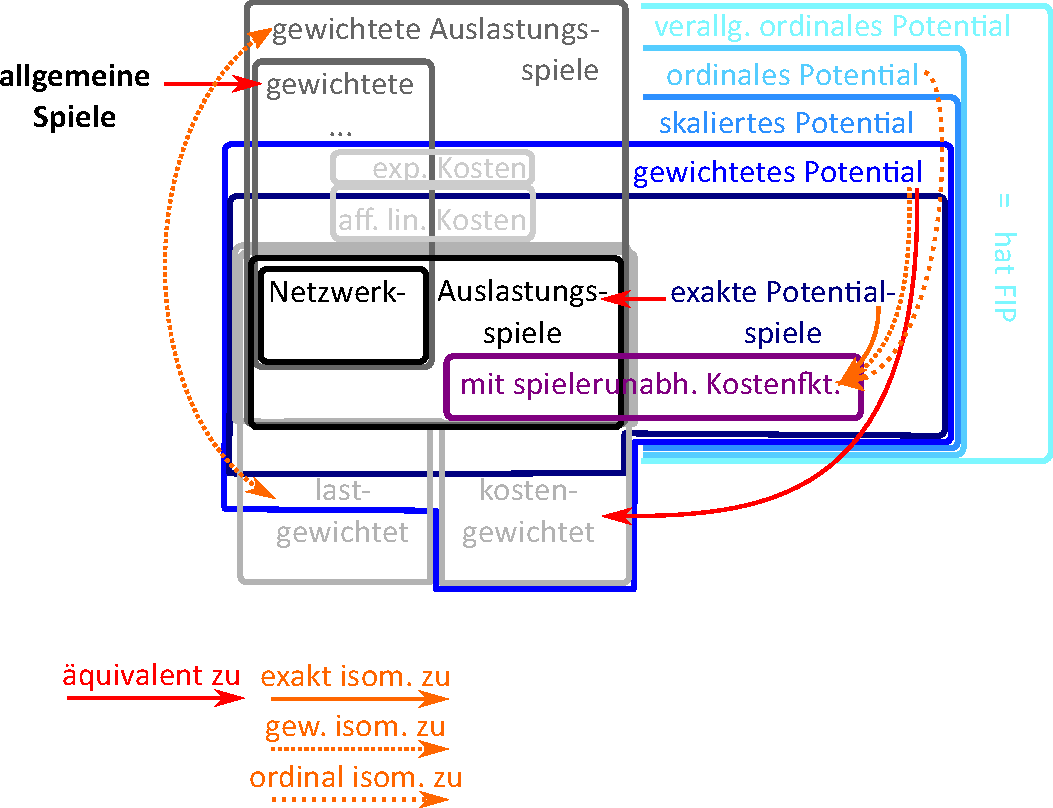
\includegraphics[width=.7\textwidth]{../Bilder/EulerDiagramm.pdf}
	\caption{Zusammenhänge zwischen den verschiedenen Spieleklassen für endliche Spiele}
\end{figure}